\documentclass[
A4paper,                % paper size A4
twoside,                % onesite or twoside printing
openright,              % doublepage cleaning ends up right side
chapterprefix=true,     % prefix for chapter marks
12pt,                   % font size
headings=normal,        % size of headings
titlepage=on            % own page for each title page
]{book}

% **************************************************
% THESIS COVER DATA
% **************************************************
% Fill in the details of your thesis: author, title, etc. 

\newcommand{\thesisTitle}{\protect {A comparative analysis across algorithmic, machine learning, and visual paradigms for the automatic detection of the perceived origin of full-body human movement}}
\newcommand{\thesisAuthor}{\protect{Fausto Martina, Romano Gabriele}}
% \newcommand{\priorstudies}{\protect{<Previous academic degree>}}
\newcommand{\thesisDate}{\the\numexpr\year-1\relax/\the\year}
\newcommand{\University}{\protect {University of Genoa}}
\newcommand{\Course}{\protect {Computer Engineering}}

\newcommand{\supervisors}{Prof. Volpe Gualtiero, Prof. Oneto Luca}
\newcommand{\cosupervisor}{<[Add co-supervisor if applicable]> }

%\newcommand{\supervisorDetails}{<Supervisor Name and Surnames, position, institution> }
%\newcommand{\cosupervisorDetails}{<[Add co-supervisor if applicable, including position and institution]> }
%\usepackage{dibrisunige-report}
%\usepackage{thesis-config}
\usepackage[protrusion=true, expansion=true]{microtype}  % Use microtype to improve readability
\usepackage{lmodern}     % Use a modern font (that is not pixelated)
\usepackage{booktabs}    % nicer horizontal rules in tables
\usepackage{emptypage}   % no headers in empty pages
\usepackage[small,hang,bf]{caption}    % caption options
\usepackage{csquotes}
\usepackage{hyperref}
\usepackage{parskip}     % paragraph spacing (suppress indentation)
\usepackage{colortbl, xcolor} % For cells colors
\usepackage{tocloft}
\usepackage{graphicx} % To fit images
\usepackage{float}
\usepackage{fancyhdr}
\usepackage{geometry}
\usepackage[utf8]{inputenc}
\usepackage{etoolbox}
\usepackage[doublespacing]{setspace}
\usepackage{anyfontsize}

% To create graphs
\usepackage{tikz}
\usepackage{pgfplots}
\usetikzlibrary{positioning}
\usepackage{diagbox}
\usepackage{slashbox}
\usepackage{subcaption}
\usepackage{titlesec}
\usepackage{chngcntr}


\usepackage{algorithm}
\usepackage[noend]{algpseudocode}

% Encodings
\usepackage{amsmath,amssymb,gensymb,textcomp}

% Better tables
% Wide tables go to https://tex.stackexchange.com/q/332902
\usepackage{array,multicol,multirow,siunitx,tabularx}

% Better enum
\usepackage{enumitem}

% Graphics
\usepackage{caption,float}

% Allow setting >max< width of figure
% 'export' allows adjustbox keys in \includegraphics
\usepackage[export]{adjustbox}


\usepackage{titletoc}


\graphicspath{{graphics/}}
\newlist{mydescription}{description}{1}
\setlist[mydescription,1]{labelindent=2em, leftmargin=2em}

\fancyhead[RO]{\nouppercase \leftmark}  % Define the header for odd and even pages
\fancyhead[LE]{}           % Define the header for odd and even pages
\fancyfoot[C]{\thepage}

\titlecontents{chapter}[0pt]
  {\addvspace{1em}}
  {\textbf{\thecontentslabel}\hspace{0.8em}\textbf} % Increase the space here (2em in this example)
  {}
  {}
%\titlecontents{chapter}[0pt]{\addvspace{0em}}{\thecontentslabel\hspace{1em}}{}{\titlerule*[1pc]{}\contentspage}
\titlecontents{section}[8pt]{\addvspace{0em}}{\thecontentslabel\hspace{0.8em}}{}{\titlerule*[0.8pc]{.}\contentspage}
%\titlecontents{subsection}[2em]{\addvspace{0em}}{\thecontentslabel\hspace{1em}}{}{\titlerule*[1pc]{}\contentspage}


% Configurations
\newcounter{memberrowno}
\setcounter{memberrowno}{0}

%\oreporttype{Thesis}
\title{A comparative analysis across algorithmic, machine learning, and visual paradigms for the automatic detection of the perceived origin of full-body human movement}
%\multiadvisor{Gualtiero Volpe}
%\multiadvisor{Luca Oneto}
\renewcommand{\headrulewidth}{0.2pt}
\renewcommand{\contentsname}{\Huge Table of contents}
\renewcommand{\listfigurename}{\Huge List of Figures}
\renewcommand{\listtablename}{\Huge List of Tables}

% --------------------------
% Customize document
% --------------------------
% Define the geometry of the document
\newgeometry {top=2.5cm, bottom=2.5cm, right=2.5cm, left=2.5cm}

\setlength{\parskip}{10pt}   % Change the default value

% hiperlinks
\hypersetup{
    colorlinks=true,          % Enable colored links
    linkcolor=black,          % Color for internal links
    urlcolor=blue,
    citecolor=blue
}
\setlength{\parskip}{10pt}   % Change the default value


%\cftsetindents{table}{-1em}{3.5em}
%\cftsetindents{figure}{-1em}{3.5em}

% Reset the figure counter at the beginning of each chapter
\counterwithin{figure}{section}
\counterwithin{table}{section}

\begin{document}
%\titleformat{\part}[display]
%  {\centering\Huge\bfseries}{\partname\ \thepart}{20pt}{\Huge}
\frontmatter
\pagestyle{empty}				    % no header nor footer
\begin{center}
    \begin{spacing}{2} % Adjust the spacing between lines
       \textbf{\large {\University}}\\
    \end{spacing}
    
    \vspace{0.5cm}

    \includegraphics[width=4cm]{logoColorized.png}
    
    \begin{spacing}{1.5} % Adjust the spacing between lines
      \textbf{\large {\Course}}\\
    \end{spacing}

    \vspace{2cm} % Adjust vertical space

    \begin{spacing}{2.4} % Adjust the spacing between lines
      \textbf{\LARGE {\thesisTitle}}
    \end{spacing}
  
    \vspace{2cm} % Adjust vertical space
  
    \begin{spacing}{1.5} % Adjust the spacing between lines
      \textbf{\large {Candidates}}\\
      {\large \thesisAuthor}\\
    \end{spacing}

    \vspace{0.5cm} % Adjust vertical space

    \begin{spacing}{1.5} % Adjust the spacing between lines
      \textbf {\large {Advisors}} \\
      {\large {Dr. \supervisor}}\\
    \end{spacing}

    \vfill
    \begin{center}
      {\large Academic year \thesisDate}
    \end{center}
\end{center}
\newpage

\pagenumbering{roman}			    % roman page numbering 
\pagestyle{plain}				    % empty header, just page number in footer

\include{chapters/acknowledgments.tex}
\section{Abstract}

A concise summary of the thesis, highlighting the main objectives, methods, findings, and conclusions. The abstract should provide readers with a clear overview of your research.\\

\newpage

\setcounter{tocdepth}{3}		% define depth of toc
\tableofcontents				% display table of contents
\newpage

\addcontentsline{toc}{section}{\textbf{List of Figures}}
\listoffigures
\newpage

\addcontentsline{toc}{section}{\textbf{List of Tables}}
\listoftables
\newpage

\section*{\Huge Acronyms}



\begin{table}[H]
    \begin{tabular}{c c}
        \textbf{MoCap} & Motion Capture Technology \\
        \textbf{MWPM} & Maximum Weight Perfect Matching \\
        \textbf{KNN} & K-Nearest Neighbors \\
        \textbf{B-SMOTE} & Borderline Synthetic Minority Over-sampling Technique \\
    \end{tabular}
\end{table}
\cleardoublepage

% --------------------------
% Main matter
% --------------------------
\mainmatter
\pagenumbering{arabic}			% arabic page numbering
%\setcounter{page}{1}			% set page counter
\pagestyle{fancy} 	            % fancy header and footer
\parskip=7pt                    % space after each paragraph
\parindent=0pt                  % suppress indentation of paragraphs

%\part{Background}
\chapter{Introduction}
The thesis consists of a summary report and a prototype system written in Python.
The dataset was sourced from the archives of Casa Paganini, the same location where artists' performances were recorded. 

\section{Context}
In sports, dance, and physical activities, motion capture technology stands as a game-changer.
It offers immense benefits for athletes and artists by revolutionizing their training methods and performance outcomes.
The use of motion capture technology goes beyond traditional training approaches.
It provides athletes with precise insights and tools to refine their techniques and improve performance.
Whether it's analyzing running styles or perfecting the fluid movements in dance routines, these technologies play a crucial role in skill enhancement.
Moreover, these tools aren't solely focused on improving performance; they also help prevent injuries by identifying potential stress points or incorrect body movements that could lead to harm.
In rehabilitation, motion capture accelerates the recovery process by monitoring movements accurately. This allows for tailored rehabilitation programs, ensuring a quicker return to peak physical condition after an injury.
What's impressive is that this technology encourages self-improvement.
It allows individuals to monitor their performances, pinpoint areas for improvement, and make necessary adjustments independently. This fosters a culture of continuous self-improvement without always relying on external expertise.
Additionally, motion capture isn't limited to professionals; it's accessible for enthusiasts and newcomers. It encourages independent learning and exploration of movement analysis, biomechanics, and performance enhancement.
In essence, motion capture technology redefines training, performance, and recovery by not only enhancing performance and preventing injuries but also empowering individuals to take charge of their own progress.


In kayaking, trunk motion stands as a critical factor influencing both injury prevention and performance enhancement \cite{kayak}.
Previous kinematic studies within this domain have predominantly occurred in controlled laboratory settings employing paddling simulators and ergometers.
However, these setups fail to authentically emulate the complexities of kayaking in a competitive water environment.
To address this limitation, a video camera-type kayak motion capture system (KMCS) was introduced, utilizing action cameras affixed to a kayak to capture markers placed on an athlete's body.

The use of Motion Capture is also employed to identify which motion features can effectively distinguish between performances of professional violinists and those of novice students, without relying on the produced sound \cite{oneto:2020}. 
In traditional music education, the predominant approach revolves around a teacher-student relationship, where the delay between a student's performance and the instructor's feedback causes a disconnect between the teacher's input and the student's auditory perception, as discussed in \cite{violino:1985}.
Given that this interaction commonly takes place during weekly classes, this aspect becomes even more significant \cite{violino:1993}.
This critical aspect of music instruction is frequently overlooked, leaving students accustomed to practicing independently without comprehending how to structure and assess their progress during solitary rehearsals.
It's important to acknowledge that prolonged periods of self-study among students can be challenging, leading to a solitary experience that frequently results in a high dropout rate \cite{violino:2011}.
To effectively tackle these challenges in music education, it is highly beneficial to consider reflective thinking and the cognitive aspects of learning.
As we can see in \cite{violino:how_we_think}, there exist four innate forms of thinking within the humnan mind and the fourth type emphasized is known as reflective thinking, a foundational aspect of what we refer to as metacognition.
Reflection isn't just a series of thoughts; it's a sequence where each thought leads to the next as its logical consequence, and each subsequent thought relates back to or builds upon its predecessors.
This underlines the importance of fostering reflective and metacognitive thinking in music education, enabling students to assess their own learning process. Employing self-regulation strategies and metacognition can enhance the outcomes of music learning.
In regard to self-regulation strategies, Nielsen \cite{violino:nielsen} investigated their application by studying how two college-level musicians monitored their learning progress. This involved observing practice behaviors, collecting verbal reports during practice sessions, and conducting retrospective debriefing reports post-practice to delve into the facets of self-directed learning.
The \cite{oneto:2020} proposes a system for automatically classifying recordings of performances by professional musicians and violin students.
This analysis will focus on two distinct scenarios, aiming to expand the findings obtained concerning different exercises and diverse violinists.
Additionally, efforts will be made to identify the most relevant movement characteristics for assessing a violinist's abilities, thereby reinforcing the significance of the obtained results.
These outcomes, besides validating the model's accuracy, will be pivotal in gaining a deeper understanding of the challenge and advocating for the utilization of this technique as a valuable support tool for students, aiding them in tracking and enhancing their individual practice at home.

In \cite{emotion_recognition} it is introduced a computational model and a system designed to automatically recognize emotions based on full-body movements.
The three-dimensional motion data capturing these movements is sourced from professional optical motion-capture systems (\textit{Qualisys}) or more affordable RGB-D sensors (\textit{Kinect} and \textit{Kinect2}).
The resulting model and system have been successfully applied in the development of serious games for helping autistic children learn to recognize and express emotions by means of their full-body movement.
Traditionally, theories of emotion have primarily focused on facial and vocal expressions, sidelining the significance of full-body movements and expressive gestures until recent years.
Limited explorations in psychology and computer systems analyzing full-body movement for emotional and expressive content existed.
Recent studies highlight advantages in expressing and recognizing emotions through full-body gestures.
For instance, from a distance, bodily cues are more perceptible than subtle facial changes.
A growing body of research in affective neuroscience underscores the role of the entire body in expressing and even subconsciously recognizing emotions.
This shift is evident in multimedia technology utilizing full-body movement across various applications.

One of the Sustainable Development Goals suggested by the United Nations Organization (ONU) is geared toward achieving universal and comprehensive healthcare coverage while reducing related inequalities, aiming to ensure that everyone enjoys good health \cite{onu}.
In line with this, it is acknowledged that inequalities contribute to millions of people with disabilities facing challenges in performing their basic daily activities.
This disparity is more pronounced among individuals from communities with fewer opportunities and resources, typically located in geographically distant areas from the necessary rehabilitation services \cite{world_report_disability}.
Among various types of disabilities, motor impairment is considered one of the primary hindrances in executing daily activities for humans, significantly impacting the individual's quality of life and those around them \cite{ida_website}.
In recent years, telemedicine and telerehabilitation have been enhanced through the implementation of diverse technologies supporting rehabilitation processes.
These innovations aim to provide necessary services to patients, reducing the need for frequent trips to major cities, where specialists, hospitals, clinics, and technologically equipped therapy centers are typically located.
\cite{riabilitazione} focuses on supporting the physical rehabilitation of upper limbs using video games and a motion capture system, primarily employing the Kinect sensor and inertial sensors for motion capture.

Cycling is one of the most widely practiced sports globally, both professionally and recreationally.
Covering long distances during a training session imposes significant metabolic and biomechanical stress on the body.
Epidemiological studies have demonstrated that cycling carries a high incidence of overuse injuries, making it one of the sports with a considerable number of yearly incidents, following basketball and soccer.
Analyzing a cyclist's posture during pedaling is crucial not only to identify biomechanical factors limiting performance but also to uncover injury predispositions.
Abnormal pelvic movements during cycling correlate with poor bike fit and related pathologies.
Employing a Motion Capture System, considered the gold standard for assessing biomechanical parameters in sports performance, our aim is to investigate variations in pelvic kinematics during different phases of the pedaling cycle.
Ten cyclists were engaged in the study, pedaling at varied cadences.
Upon data collection, pelvic kinematic parameters were analyzed.
Through statistical analysis, the three different pedaling conditions were compared.
This study \cite{ciclismo} revealed that the lowest pelvic oscillation occurs at 90 revolutions per minute (rpm).
Despite not being the lowest pedaling frequency, this rate proves to be the safest in preventing injuries and the most comfortable for cyclists.


\section{Starting point and problem statement}
Currently the method for automated analysis of body movement consists of an approach involving transferable-utility cooperative games on graph \cite{kolykhalova:2020}.
A Motion Capture dataset is originated by recording with 13 infra-red cameras, two professional dancers that were equipped with 64 infra-red reflective markers, 5 accelerometers and 1 microphone.
Then the perceived Origin of Movement are manually annotated by experts in the field.
By using the native software “Qualisys Track Manager” have been computed the trajectories of each point and tracked across the whole timeframe of the sample.\\
The output of the software is a highly precise description of the trajectories of either 64, 62 or 41 markers based on the version of the capture system. 
Then the number of markers has been compressed by clustering and mapping the markers based on a scheme that uniquely maps the human skeletal structure, resulting in 20 points, that from now will be called $joint$.
By iterating this process over each sample of the dataset a list of 36 labeled timeseries is obtained.\\
From here three kinds of movements features are calculated for each joint: speed, acceleration and angular momentum.
The analysis is performed separately for each kind of feature.
Then a first graph is created by linking each joint that is physically connected with another.
A weight for each arc (or edge) is assigned based on the similarity of the selected feature calculated on the two joints.
Henceforth a clustering algorithm is applied on the graph to further reduce the analysis on the edges that are outliers and fall across two different clusters.
Then the weight of the edge is split between the two joints and the Shapley value approach is used as solution to the mathematical game built with the weighted vertices.\\

Results are validated with an online survey, where have been asked to users at various level of self-assessed proficiency, 
to select one or two vertices of the skeletal structure as the origin of movement.
They were given hints in three diverse ways by highlighting the joints, either, 
with the highest Shapley values, with the maximum speed, or randomly chosen. 
This study has proven that the most expert users consistently chose as origin of movement the one suggested by Shapley values. 



\section{Thesis's structure}

\section{Origins and technological rise of Motion Capture}
The origin of motion capture can be traced back to the mid-20th century when rudimentary methods were employed, 
often involving manual tracking of key points on a subject's body. 
The introduction of marker-based MoCap in the 1970s marked a significant advancement. 
This technique involved attaching reflective markers to specific body points, which were then tracked by cameras to reconstruct the subject's movement in a digital environment. 
The example depicted in Figure \ref{fig:mocap_scene} illustrates two performers at the top engaged in a ball game, throwing it from one side to the other. Below, you can see the corresponding digital reconstruction. 
Technically, only the markers are automatically recognized, while the connections between markers are manually made, so these are later added.
\begin{figure}[H]
    \centering
    \includegraphics[width=0.75\textwidth]{bodyMarkersExampleImage.png}
    \includegraphics[width=0.75\textwidth]{bodyMarkersExampleMoCap.png}
    \caption{Video frame and MoCap scene with infrared cameras and markers}
    \label{fig:mocap_scene}
\end{figure}
\vspace{-1.5\baselineskip}
However, marker-based MoCap had limitations, including occlusion 
(when markers were hidden from view), inaccuracies, and the need for time-consuming calibration processes. 
These limitations led to the development of markerless MoCap technology. 
Markerless MoCap uses computer vision algorithms to track and reconstruct movement without the need for physical markers. 
This approach relies on complex algorithms that can identify and track features of the human body, 
such as joint positions and skeletal structure, from video footage.


\section{Motivation}
While relationships between emotions and facial expressions or voice changes have been widely explored, 
leading to the availability of feasible methods for real-time automatic analysis, 
full-body movement has not been equally investigated. 
Various studies have shown great potential for inferring about emotions and many other human activities \cite{Bachmann:2020, preiler:2023}. 
Being able to automatically analyse the origin of movement could improve human performances, 
prevent injuries, promote physical activity, develop cognitive and motor rehabilitation strategies \cite{piana:2016}. 

For this reason, the research in human movement has branches in various fields of study such as biomechanics and neuroscience \cite{vaessen:2019}, 
experimental psychology, and theories from the arts and humanities \cite{camurri:2016}. 

The progress made in this field still does not allow a complete and robust classification of the origin of movement, in an automated way, 
because this relies mainly on arbitrary thresholds to distinguish between different origins and current state of the body, 
like if it is moving or standing still. 
For example, to recognize the instant when a movement starts it is required to manually tune 
minimum speed values that are difficult to automate and generalize for every context. 

Furthermore in movement recognition there are a lot of mid-level features, like the joint angles,
or the limb trajectories or the body segment coordination, which can be extracted and exploited by a comprehensive algorithm 
that weights every feature in an optimize manner, resulting in improved accuracy over all the possible approaches 
that work on them individually, because it could take into account the possible interactions and dependencies between them. 
An holistic approach in this way could leverage the complementary informations present in each feature by weighting them 
based on their relative importance. 
One last point to take into consideration is that algorithms based on single features could end up in overfitting the data
while the comprehensive one has more generalization capability. 

This research aims to contribute to the design of accurate and robust systems for the automated analysis of the origin of movement
by exploiting both the current techniques of analysis and the emerging ML approaches, 
which have become feasible thanks to advancements in computational capabilities of modern machines. 

\chapter{State of Art}
Currently the method for automated analysis of body movement consists of an approach involving transferable-utility cooperative games on graph \cite{kolykhalova:2020} that has been summed up below:  
\begin{enumerate}
    \item {A Motion Capture dataset is originated by recording with 13 infra-red cameras. two professional dancers that were equipped with 64 infra-red reflective markers, 5 accelerometers and 1 microphone.} 
    \item{The perceived Origin of Movement are manually annotated by experts in the field.} 
    \item{With the native software “Qualisys Track Manager” have been computed the trajectories of each point.}  
    \item{Joints are created according to the human skeletal structure and then clustered into a set of 20 points.} 
    \item{Then the Shapley value approach is used as solution to the mathematical game built with the weighted vertices.} 
\end{enumerate}
Results are validated with an online survey, where have been asked to users at various level of self-assessed proficiency, 
to select one or two vertices of the skeletal structure as the origin of movement.
They were given hints in three diverse ways by highlighting the joints, either, 
with the highest Shapley values, with the maximum speed, or randomly chosen. 
This study has proven that the most expert users consistently chose as 
origin of movement the one suggested by Shapley values. 

\section{Origin of Movement}
\chapter{Proposed Approach}
Our work builds upon certain aspects of the previous research while introducing a novel and more innovative method for predicting movement origins using machine learning. 
Similar to the previous approach, the pipeline to reach the 20-joints skeleton remains the same (see Sections \ref{sec:orig_markers}, \ref{sec:reduced_markers}).

We chose to utilize an ensamble of some movements from the previous dataset (the one used in \cite{kolykhalova:2020}), enriching the number of samples from other internal resources provided by Casa Paganini \cite{casaPaganini}. 
This choice has been motivated by the necessity to have many short samples that clearly present an origin of movement instead of few samples that are hard to infer in terms of origin of movement, in order to 
reach a high-quality data that can be used in machine learning techniques that will be explained in Chapter \ref{chap:ml_method}.\\
Since we started from the previous work which was based on game theory and the concept of Shapley values in our approach we considered that there is not a clear contribution in terms of added value derived from nodes cooperation. 
Therefore, we opted for WDC (Weighted Degree Centrality) to determine the perceived origin of the movement for the algorithmic approach.\\
Furthermore for visualization purposes we implemented a method to prevent inconsistent coloring behaviours among clusters over time, by introducing a novel cluster stabilization algorithm. 

\section{Roadmap}
From the starting point of our work \cite{kolykhalova:2020}, we re-implemented, improved and modified it to compare the method for identifying the origin of movement obtained based on graphs with our new machine learning-based approach.
The roadmap of this thesis can be outlined as follows: \\
The dataset was initially acquired through manual annotation of movement origins in numerous MoCap videos. 
The results were validated by achieving consensus among multiple annotators. 
Additionally, markers for videos lacking previous labeling were manually assigned and subsequently compressed into clusters.
The central objectives of this thesis encompass the development of:
\begin{itemize}
    \item \textbf{Cluster Stabilization Algorithm} which ensure that clusters, which represent groups of related markers or joints, maintain their consistency and coherence over time. 
    \item \textbf{Graph-based Procedure} to recognize the Origin of Movement by identifying key nodes that play pivotal roles in the motion analysis using an algorithmic method.
    \item \textbf{Machine Learning Approach} to identify the most promising edge of a the skeletal model by finding patterns in data without an algorithmic approach.
\end{itemize}
Given the multifaceted objectives, two parallel pipelines were developed.\\
The first pipeline included the following steps:
\begin{itemize}
    \item Smoothing the time series of each movement using two classical smoothing algorithms.
    \item Extracting physical measurements from the smoothed data.
    \item Applying cosine similarity to pairs of joints linked by arcs based on a model of physical joints in the human body.
    \item Clustering joints for each frame of the movement.
    \item The primary objective here was the temporal stabilization of cluster color changes.
    \item Formation of a second graph with nodes at cluster borders, connected to other clusters. These nodes are weighted based on their connections and ranked across all frames.
\end{itemize}
The second pipeline involved:
\begin{itemize}
    \item Normalizing the dataset in terms of segment length (Time series Sampling), performer's body structure (Skeleton Barycenter and Joints Distance), and the entire trajectory of the movement.
    \item Extracting a wide range of relevant features from the normalized dataset.
    \item Using these features to train a machine learning model.
    \item Evaluating the model's performance using various metrics.
\end{itemize}
Finally, the results from each pipeline are compared.

\clearpage
\begin{figure}[H]
    \centering
    \includegraphics[width=\textwidth,height=\textheight,keepaspectratio]{Walkthrough.png}
    \caption{Roadmap of this Thesis}
    \label{fig:walktrough}
\end{figure}
\chapter{Theoretical framework}
\label{sec:theoretical_framework}

\section{Graph theory}
This section contains definitions, notation and concepts related to Graph Theory according
to \cite{graph_theory:2010}. \\
Graph theory deals with connection amongst vertices by edges. \\
Graphs are the foundation of many day to day processes and concepts, as they provide a convenient
and intuitive way of representing objects.

\subsection{Simple graphs}
A \textbf{simple graph} \textit{G} consists of a non-empty finite set \textit{V(G)} of elements called \textbf{vertices}
(or \textbf{nodes}), and a finite set \textit{E(G)} of distinct unordered pairs of distinct elements of \textit{V(G)}
called \textbf{edges}. We call \textit{V(G)} the \textbf{vertices set} and \textit{E(G)} the \textbf{edge set} of G.
An edge $\{\textit{v}, \textit{w}\}$ is said to join the vertices v and w, and is usually abbreviated to vw. For example, Figure~\ref{fig:simple_graph} represents the simple graph G whose vertex set \textit{V(G)} is $\{\textit{u}, \textit{v}, \textit{w}, \textit{z}\}$, and whose
edge set \textit{E(G)} consists of the edges \textit{uv}, \textit{uw}, \textit{vw} and \textit{wz}. 

\begin{figure}[H]
    \centering
    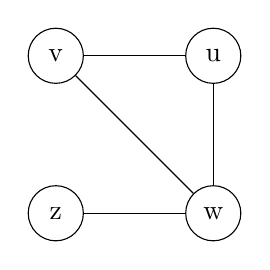
\begin{tikzpicture}
      % Disegno dei nodi
      \node[circle, draw, minimum size=0.7cm] (v) at (0,0) {v};
      \node[circle, draw, minimum size=0.7cm] (u) at (2,0) {u};
      \node[circle, draw, minimum size=0.7cm] (w) at (2,-2) {w};
      \node[circle, draw, minimum size=0.7cm] (z) at (0,-2) {z};
      
      % Disegno degli archi
      \draw (u) -- (v);
      \draw (u) -- (w);
      \draw (v) -- (w);
      \draw (w) -- (z);
    \end{tikzpicture}
    \caption{A simple graph}
    \label{fig:simple_graph}
\end{figure}

\subsection{Adjacency}
We say that two vertices \textit{v} and \textit{w} of a graph \textit{G} are \textbf{adjacent} if there is an edge \textit{vw} joining them, and the vertices \textit{v} and \textit{w} are then \textbf{incident} with such an edge. \\
Similarly, two distinct edges \textit{e} and \textit{f} are \textbf{adjacent} if they have a vertex in common (see Figure \ref{fig:adiacency}).

\begin{figure}[H]
    \centering
    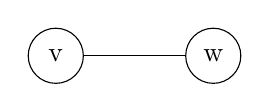
\begin{tikzpicture}
      % Primo grafo
      \node[circle, draw, minimum size=0.7cm] (v) at (0,0) {v};
      \node[circle, draw, minimum size=0.7cm] (w) at (2,0) {w};
      \draw (v) -- (w);
    \end{tikzpicture}
    \quad % Spazio tra i grafi
    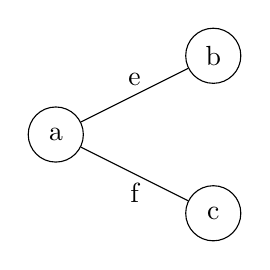
\begin{tikzpicture}
      % Secondo grafo
      \node[circle, draw, minimum size=0.7cm] (a) at (0,0) {a};
      \node[circle, draw, minimum size=0.7cm] (b) at (2,1) {b};
      \node[circle, draw, minimum size=0.7cm] (c) at (2,-1) {c};
      \draw (a) -- node[above] {e} (b);
      \draw (a) -- node[below] {f} (c);
    \end{tikzpicture}
    \caption{Adjacent vertices and adjacent edges}
    \label{fig:adiacency}
\end{figure}

\subsection{Weighted Degree Centrality}
\label{subsec:weighted_degree}
Weighted degree centrality is a measure used in network analysis to quantify the importance or centrality of a node in a network, taking into account the weights of the edges connected to that node. 
Unlike traditional degree centrality, which only considers the number of connections (edges) a node has, weighted degree centrality considers the strengths or weights associated with those connections.
For a given node, calculate its weighted degree by summing up the weights of all the edges connected to that node. In mathematical terms, it can be expressed as:
\begin{equation}
  WDC(v) = \sum_{i=1}^{N} w_{vi}
\end{equation}
Where \textit{v} is a vertex in the graph and \textit{N} is the number of vertices.

\subsection{Matrix representations}
One approach to representing a graph is through the use of matrices, especially when dealing with large graphs that may not be well-suited for diagram-based representations.\\
Let's consider a graph \textit{G} with \textit{n} vertices and \textit{m} edges. \\
An \textbf{adjacency matrix A} is the $n \times n$ matrix whose \textit{ij}-th entry is the number of edges joining vertex \textit{i} and vertex \textit{j}. \\
If, in addition, the edges are labelled $\{1, 2, \dots, m\}$, its \textbf{incidence matrix M} is the $n \times m$ matrix whose \textit{ij}-th entry is 1 if vertex \textit{i} is incident to edge \textit{j}, and 0 otherwise. \\
An example of this is given in Figure \ref{fig:matrix_representations}.

\begin{figure}[H]
    \centering
    \begin{minipage}{0.5\textwidth}
        \centering
        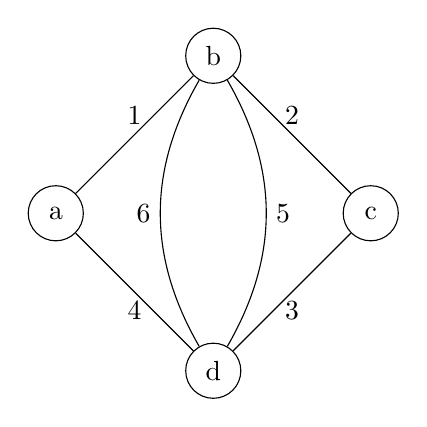
\begin{tikzpicture}
            % Nodi
            \node[circle, draw, minimum size=0.7cm] (a) at (0,0) {a};
            \node[circle, draw, minimum size=0.7cm] (b) at (2,2) {b};
            \node[circle, draw, minimum size=0.7cm] (c) at (4,0) {c};
            \node[circle, draw, minimum size=0.7cm] (d) at (2,-2) {d};
          
            % Archi
            \draw (a) edge node[pos=0.5, below] {4} (d);
            \draw (a) edge node[pos=0.5, above] {1} (b);
            \draw (b) edge[bend left] node[pos=0.5, right] {5} (d);
            \draw (b) edge[bend right] node[pos=0.5, left] {6} (d);
            \draw (b) edge node[pos=0.5, above] {2} (c);
            \draw (c) edge node[pos=0.5, below] {3} (d);
        \end{tikzpicture}
    \end{minipage}%
    \begin{minipage}{0.5\textwidth}
        \[
        A = \begin{bmatrix}
        0 & 1 & 0 & 1 \\
        1 & 0 & 1 & 2 \\
        0 & 1 & 0 & 1 \\
        1 & 2 & 1 & 0
        \end{bmatrix}
        \]
        
        \[
        M = \begin{bmatrix}
        1 & 0 & 0 & 1 & 0 & 0 \\
        1 & 1 & 0 & 0 & 1 & 1 \\
        0 & 1 & 1 & 0 & 0 & 0 \\
        0 & 0 & 1 & 1 & 1 & 1
        \end{bmatrix}
        \]
    \end{minipage}
    \caption{Graph \textit{G} with its adjacency \textit{A} and incidence \textit{M} matrices}
    \label{fig:matrix_representations}
\end{figure}


\subsection{Bipartite graphs}
If the vertex set of a graph \textit{G} can be split into two disjoint sets \textit{A} and \textit{B} so that each
edge of \textit{G} joins a vertex of \textit{A} and a vertex of \textit{b}, then \textit{G} is a \textbf{bipartite graph}. \\
Alternatively, a bipartite graph is one whose vertices can be coloured red and blue in such a way that each edge joins a red vertex (in \textit{A}) and a blue vertex (in \textit{B}). \\

\begin{figure}[H]
    \centering
    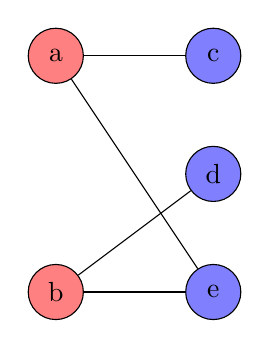
\begin{tikzpicture}[every node/.style={circle, draw, minimum size=0.7cm}]
        % Livello superiore
        \node (A) at (3,0) [fill=red!50] {a};
        \node (B) at (3,-3) [fill=red!50] {b};
        
        % Livello inferiore
        \node (C) at (5,0) [fill=blue!50] {c};
        \node (D) at (5,-1.5) [fill=blue!50] {d};
        \node (E) at (5,-3) [fill=blue!50] {e};
        
        % Collegamenti
        \draw (A) -- (C);
        \draw (A) -- (E);
        \draw (B) -- (D);
        \draw (B) -- (E);
    \end{tikzpicture}
    \caption{A simple bipartite graph}
    \label{fig:bipartite}
\end{figure}



\subsection{Bipartite graphs with matching}
A \textbf{bipartite graph with matching} is a bipartite graph in which there is a set of edges selected in such a way that no node is shared among the edges of the matching.
In other words, each node is involved in at most one edge of the matching. \\
This means that if the number of vertices in \textit{A} and \textit{B} is different, at least one vertex will have no connection to another vertex (see Figure \ref{fig:match_1}). \\
If there is the same number of vertices in both \textit{A} and \textit{B}, every vertex is connected to another vertex (see Figure \ref{fig:match_2}). \\

\begin{figure}[H]
  \centering
  \begin{subfigure}{0.48\linewidth}
    \centering
    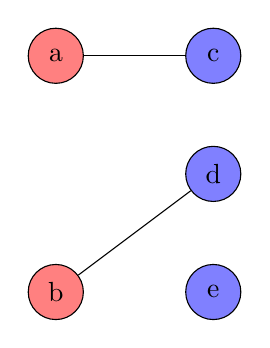
\begin{tikzpicture}[every node/.style={circle, draw, minimum size=0.7cm}]
      % Livello superiore
      \node (A) at (3,0) [fill=red!50] {a};
      \node (B) at (3,-3) [fill=red!50] {b};

      % Livello inferiore
      \node (C) at (5,0) [fill=blue!50] {c};
      \node (D) at (5,-1.5) [fill=blue!50] {d};
      \node (E) at (5,-3) [fill=blue!50] {e};

      % Collegamenti
      \draw (A) -- (C);
      \draw (B) -- (D);
    \end{tikzpicture}
    \caption{}
    \label{fig:match_1}
  \end{subfigure}
  \hspace{0.02\linewidth}
  \begin{subfigure}{0.48\linewidth}
    \centering
    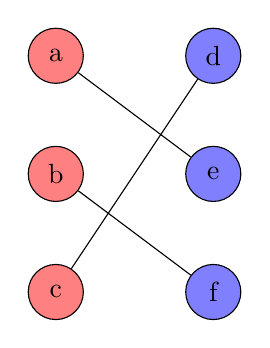
\begin{tikzpicture}[every node/.style={circle, draw, minimum size=0.7cm}]
      % Livello superiore
      \node (A) at (3,0) [fill=red!50] {a};
      \node (B) at (3,-1.5) [fill=red!50] {b};
      \node (C) at (3,-3) [fill=red!50] {c};

      % Livello inferiore
      \node (D) at (5,0) [fill=blue!50] {d};
      \node (E) at (5,-1.5) [fill=blue!50] {e};
      \node (F) at (5,-3) [fill=blue!50] {f};

      % Collegamenti
      \draw (A) -- (E);
      \draw (B) -- (F);
      \draw (C) -- (D);
    \end{tikzpicture}
    \caption{}
    \label{fig:match_2}
  \end{subfigure}
  \caption{Bipartite graph}
\end{figure}

\subsection{Maximum Weight Perfect Matching}
\label{sec:MaxWPM}
The Maximum Perfect Weight Matching is an optimization problem concerning graphs.
The graphs in question are bipartite, meaning the vertices can be divided into two distinct sets in such a way that all edges of the graph connect vertices from different sets, with no edges connecting vertices within the same set.
Additionally, these graphs are undirected, meaning the relationship between two nodes is bidirectional, in other words, the edge connecting node A to node B automatically implies the existence of the edge connecting node B to node A. \\
In the MaxWPM problem, the vertices represent elements to be paired, and the edges represent possible connections between these elements. 
Each edge is associated with a weight that represents the value or importance of the pairing between the connected vertices.\\
The goal is to find a perfect matching, which is a set of edges in which every node is connected to exactly one other node, with no overlaps or isolated nodes, while maximizing the total weight of the edges in the matching.
The total weight is the sum of the weights of the edges included in the matching.
The weights of the edges are collected in a matrix called a \textit{utility matrix}.\\
The utility matrix will be a square matrix because the number of nodes in the two distinct sets is the same.
The rows could represent the nodes in the first set, while the columns could represent the nodes in the second set, or vice versa.
The element (\textit{i}, \textit{j}) of the matrix represents the weight of the edge connecting vertex \textit{i} to vertex \textit{j}. 


A MaxWPM problem using an utility matrix can be transformed into a \textbf{Minimum Weight Perfect Matching} problem.
This can be achieved by introducing an auxiliary matrix, referred to as the \textit{cost matrix}.
The cost matrix is essentially a duplicate of the utility matrix, but with all its elements negated.

\subsection{Brute Force Algorithm}
The BF can be a possible approach to solve the MaxWPM problem for bipartite graphs.
However, it's important to note that the BF has exponential time complexity, specifically, its time complexity grows exponentially with the number of vertices in the graph.
This is because the BF examines all possible combinations of matchings within the bipartite graph to find the one with the maximum weight.\\
If the graph has \textit{n} vertices in both the first and second partitions, there are \textit{n}!\ possible matchings.
Each matching requires \textit{O}(\textit{n}) time to be computed because you need to check that it is a perfect matching and calculate its total weight.
Therefore, the overall complexity of the algorithm is on the order of \textit{O}(\textit{n}!$\cdot$\textit{n}). \\
Since the complexity grows rapidly as \textit{n} increases, it quickly becomes impractical for large-sized graphs. \\

The operation of the BF for MinWPM problems can be summerized in these 3 steps:

\begin{enumerate}
    \item {Compute the cost matrix for the considered bipartite graph with \textit{n} vertices in each partition.}
    \item {Compute the total cost of all the \textit{n}!\ permutations.}
    \item {Choose the assignment with the lowest total cost.}
\end{enumerate}


\subsection{Hungarian Matching Algorithm}

The HM, also called the Kuhn-Munkres algorithm, is a \textit{O}($\textit{n}^3$) algorithm that can be used to find MaxWPM in bipartite graphs with \textit{n} vertices for each partition, which is sometimes called the assignment problem.
As previously demonstrated in the Brute Force algorithm, maximum-weight perfect matching problems using the utility matrix can be converted into MinWPM problems using the cost matrix. 
We will describe the application of the HM to address Minimum Weight Perfect Matching problems. \\

The operation of the HM for MinWPM problems can be summerized in these 6 steps:
\begin{enumerate}
    \item {Compute the cost matrix for the considered bipartite graph with \textit{n} vertices in each partition.}
    \item {Subtract the smallest entry in each row from all the other entries in the row. This will make the smallest entry in the row now equal to 0.}
    \item {Subtract the smallest entry in each column from all the other entries in the column. This will make the smallest entry in the column now equal to 0.}
    \item {Draw lines through the row and columns that have the 0 entries such that the fewest lines possible are drawn.}
    \item {If there are n lines drawn, an optimal assignment of zeros is possible and the algorithm is finished. If the number of lines is less than n, then the optimal number of zeroes is not yet reached. Go to the next step.}
    \item {Find the smallest entry not covered by any line. Subtract this entry from each row that isn’t crossed out, and then add it to each column that is crossed out. Then, go back to Step 3.}
\end{enumerate}



\section{Game theory}
Game theory is a type of decision theory in which one’s choice of action is determined after taking
into account all possible alternatives available to an opponent playing the same game, rather than just
by the possibilities of several outcome results. \\
Game theory does not insist on how a game should be played but tells the procedure and principles by which action should be selected.
Thus it is a decision theory useful in competitive situations. \\
Game is defined as an activity between two or more persons according to a set of rules at the end of
which each person receives some benefit or suffers loss. The set of rules defines the game.
Going through the set of rules once by the participants defines a play.
\\

The following sections contains notations and properties accordind to \cite{game_theory:2020}.

\subsection{Properties of a Game}
\begin{enumerate}
    \item {There are finite numbers of competitors called \textit{players}.}
    \item {Each player has a finite number of possible courses of action called \textit{strategies}.}
    \item {All the strategies and their effects are known to the players but player does not know which
    strategy is to be chosen.}
    \item {A game is played when each player chooses one of his strategies. The strategies are assumed
    to be made simultaneously with an outcome such that no player knows his opponents strategy
    until he decides his own strategy.}
    \item {The game is a combination of the strategies and in certain units which determines the gain or
    loss.}
    \item {The figures shown as the outcomes of strategies in a matrix form are called \textit{pay-off matrix}.}
    \item {The player playing the game always tries to choose the best course of action which results in
    optimal pay off called \textit{optimal strategy}.}
    \item {The expected pay off when all the players of the game follow their optimal strategies is
    known as \textit{value of the game}. The main objective of a problem of a game is to find the value
    of the game.}
    \item {The game is said to be \textit{fair} game if the value of the game is zero otherwise it's known as \textit{unfair}.}
    \item {A \textit{coalition} is a subset of the players \textit{n}, whereas a \textit{grand coalition} is the
        set \textit{n} of all players. The purpose of a coalition is to coordinate strategies and divide the
        total payoff among all the players.}
\end{enumerate}


\subsection{Cooperative Games}
A cooperative game is a situation in which players interact together to achieve a common goal.
In the context of a cooperative game, players aim to maximize the overall outcome by collaborating, communicating, and coordinating their actions.
The primary objective is to achieve a result in which all players benefit, working together to overcome challenges or issues.


\subsection{Non-cooperative Games}
A non-cooperative game is a situation in which players act independently and without direct communication or coordination with other players.
In a non-cooperative game, each player seeks to maximize their individual gain without necessarily considering the effect of their actions on other players.
The main goal is to achieve the best personal outcome, even at the expense of other participants, without considering direct collaboration.


\section{Machine Learning Theory}
\label{subsec:ML}

ML deals with the ability of a system to improve its performance through experience, without being explicitly programmed.
It also serves as the foundation for numerous everyday applications and concepts, 
as it provides a powerful and efficient way to address complex challenges, make data-driven decisions, 
and develop intelligent systems that can learn and adapt autonomously.\\

Diving deeper into this concept, one critical aspect is the role of hyperparameters. 
Hyperparameters are settings or configurations that guide the learning process of ML algorithms. 
They act as the levers that fine-tune the behavior of these algorithms, influencing their performance, accuracy, and generalization capabilities.\\
Hyperparameters encompass a wide range of choices, such as the learning rate in gradient descent, the depth of a decision tree, the number of hidden layers in a neural network, or the number of clusters in a k-means clustering algorithm. 
Selecting the right hyperparameters can be a challenging and often iterative task, as they significantly impact the model's ability to capture underlying patterns in data.\\
The process of hyperparameter tuning involves experimenting with different combinations of values, assessing the model's performance using techniques like cross-validation, and iteratively adjusting the hyperparameters to optimize the model's accuracy and generalization. 
This fine-tuning is crucial to ensure that the ML model not only fits the training data well but also performs effectively on unseen data.
Moreover, the choice of hyperparameters is problem-dependent, and there's no one-size-fits-all solution. 
It requires a deep understanding of the algorithm, the dataset, and the specific problem at hand.saisi

\subsection{Classifier}
\label{subsec:classifier}

A mathematical \textbf{Classifier} is a model that takes an input dataset and assigns each data point to a class or category. 
The mathematical formulation of a classifier can vary depending on the algorithm used. 
Suppose we have a training dataset represented as pairs (\textit{$\overline{x}$}, \textit{y}), where \textit{$\overline{x}$} is a vector of data features, and \textit{y} is the associated class label.
The \textit{y} is a categorical (can take a fixed, number of possible values) variable that categorizes between two or more classes ('dog', 'cat', 'bird'), while in a regression problem it is a continuous variable.
Our goal is to find a function \textit{f}(\textit{$\overline{x}$}) that maps the feature vectors \textit{$\overline{x}$} to class labels \textit{y}. \\

A \textbf{Binary Classification Problem} is a specific type of classification problem where the goal is to categorize input data into one of two distinct classes or categories. 
These two classes are typically referred to as the positive class and the negative class, and the task is to assign each data point to one of these two classes based on its features or attributes.
\begin{figure}[H]
  \centering
  \includegraphics[width=0.6\linewidth]{graphics/BinaryClassification.png}
  \caption{Binary Classification example}
  \label{fig:bin_classification}
\end{figure}

\subsection{K-Nearest Neighbors}
\label{subsec:KNN}

The \textbf{KNN} algorithm is a supervised ML algorithm used for classification and regression tasks.
It is a simple and intuitive algorithm that makes predictions based on the similarity between a data point and its k-nearest neighbors in a training dataset.
The \textit{k} in \textit{k}-nearest neighbors refers to the number of items that the algorithm uses to make its prediction whether its a classification problem or a regression problem.
In Figure \ref{fig:knn} we can see a test sample represented by a green dot and we want to classify 
it either as a blue square or a red triangle based on a KNN algorithm, the decision depends on the value of \textit{k}, which determines how many nearest neighbors we consider.\\
When \textit{k} = 3 (solid line circle), the green dot is assigned to the category that has the majority among its three nearest neighbors. 
In this case, if there are 2 red triangles and only 1 blue square inside the inner circle, the green dot is classified as a red triangle. \\
When \textit{k} = 5 (dashed line circle), the green dot is assigned to the category with the majority among its five nearest neighbors. 
If there are 3 blue squares and 2 red triangles inside the outer circle, the green dot is classified as a blue square.
\begin{figure}[H]
    \centering
    \includegraphics[width=0.55\linewidth]{graphics/KNeighbours.png}
    \caption{KNN algorithm with \textit{k} = 3 and \textit{k} = 5}
    \label{fig:knn}
\end{figure}

The choice of distance metric is a critical aspect of the KNN algorithm, and while it's not typically considered a hyperparameter, it significantly influences the model's performance and outcomes. 
The selection of a specific distance metric can have a substantial impact, especially when dealing with datasets of varying sizes and dimensions. \\
If we consider for example two data points \textit{p}, \textit{q} in \textit{n}-dimensional space, there are various distance metrics that can be used to find the neighbors.\\
Among the different  most common is the Euclidean distance: 
\begin{equation}
    Euclidean(p,q) = \sqrt{\sum_{i=1}^{n} (p_i - q_i)^2}
    \label{formula:distance}
\end{equation}

\subsection{Borderline Synthetic Minority Over-sampling Technique}
\label{subsec:borderline}

\textbf{Oversampling} is a technique used in the field of imbalanced ML to address the problem of class imbalance. 
Class imbalance occurs when one class in a classification problem has significantly fewer instances than another class. 
This imbalance can lead to biased models that perform poorly on the minority class (the class with fewer instances) because the model tends to be biased towards the majority class.\\
The concept of oversampling involves increasing the number of instances in the minority class by generating synthetic or duplicate samples. 
The goal is to balance the class distribution, making the minority class more comparable in size to the majority class. 
A synthetic sample can be generated duplicating randomly another sample of the minority class or considering its underlying data distribution (ADASYN \cite{adasyn:2008}).
This could result in a performance improvement of ML models by providing them with more information about the minority class.\\
The SMOTE generates synthetic samples by interpolating between neighboring minority class instances using an underlying KNN model.\\

The \textbf{B-SMOTE} \cite{Han2005BorderlineSMOTEAN:2005}, is a vairant of the SMOTE that focuses on generating synthetic samples only for the boundary instances, which are the minority class instances close to the majority class. 
This approach aims to concentrate on the regions of the dataset that are near the decision boundary between classes. \\
The model internally fits two instances of KNN with different \textit{k} parameters (\textit{k-neighbors}, \textit{m-neighbors}): one instance to defines the neighborhood of samples to generate the synthetic samples.
The other instead is used to determine if a minority sample is in \textit{danger}. A \textit{sample in danger} is one near to the boundary between two or more classes.

In the illustrated scenario depicted in Figure \ref{fig:bordSMOTEnotApplied}, the task involves categorizing two distinct categories of network traffic: 
one being malicious (depicted in red), the other representing legitimate traffic (shown in blue), and the decision boundaries are the same color meshes.
The distribution of malicious traffic is more sparse and rare compared to legitimate traffic, this means that the classifier has been trained on an imbalanced dataset. 
The primary objective of the classification is to maximize the detection of malicious traffic, even if it entails misclassifying some instances of legitimate traffic. 
B-SMOTE is a possible solution for this scenario, where the two classes are significantly imbalanced, and the weight of legitimate traffic in the classification process could be overwhelming.

The application of the B-SMOTE algorithm facilitates class rebalancing by generating synthetic data points in the boundary regions between the classes concentrated in proximity of the decision boundary.
In Figure \ref{fig:bordSMOTEApplied}, the depicted image showcases the ultimate outcome achieved following the retraining of the classifier. 
The retraining process maintained the same parameters but employed a dataset that has been more uniformly balanced.
The synthetic samples generated by B-SMOTE are represented as light-red dots.
\begin{figure}[H]
  \centering
  \begin{subfigure}{0.45\linewidth}
    \includegraphics[width=\linewidth]{graphics/BordSMOTE_no.png}
    \caption{}
    \label{fig:bordSMOTEnotApplied}
  \end{subfigure}
  \hspace{0.01\linewidth}
  \begin{subfigure}{0.45\linewidth}
    \includegraphics[width=\linewidth]{graphics/BordSMOTE_yes.png}
    \caption{}
    \label{fig:bordSMOTEApplied}
  \end{subfigure}
  \caption{Visual representation of B-SMOTE algorithm applied on a dataset}
\end{figure}

However The B-SMOTE algorithm, like any other method, has its limitations and drawbacks:
\begin{itemize}
  \item \textbf{Risk of Overfitting:} In the provided example, the malicious data was generated using a normal distribution, while the legitimate data was generated using a uniform distribution.
  This means that the second classification fits better the underlying distribution without any a-priori assumption.
  But in some cases depending on the choice of borderline examples, 
  B-SMOTE may introduce a bias towards certain patterns or classes in the synthetic samples, which can affect the model's generalization.
  It can potentially lead to overfitting, especially when it generates a large number of synthetic samples in the borderline region. 
  This may cause the model to perform exceptionally well on the training data but poorly on unseen data.
  \item \textbf{Computationally intensive:} It can require high hardware resources, especially in high-dimensional spaces, as it involves calculating distances between data points. 
  This can lead to longer training times, making it less suitable for large datasets.
  \item \textbf{Designed for Clearly Separable Datasets:} It is designed for datasets with clear class boundaries and is most effective when the borderline instances are well-defined. 
  In cases where class separation is not distinct, it may not provide substantial benefits.
\end{itemize}
So in general, even if it aims to improve the classification of the minority class, there is no guarantee that it will always lead to better results.

\subsection{Random Forest Classifier}
\label{subsec:RF}

A \textbf{Decision Tree} (DT) is a non-parametric supervised learning algorithm, which is utilized for both classification and regression tasks. 
It has a hierarchical, tree structure, which consists of a internal nodes, leaf nodes and branches.
From the root node, splitting criterias are applied on the samples creating branches and child nodes that lead to leaf nodes which represent the final classification of the tree.
The most common impurity measure used to quantify the impurity of a dataset is the Gini criterion:
For a set of items with \textit{J} classes and relative frequencies $p_{i}$, $i \in {1,2,...,J}$ 
the probability of choosing an item with label $i$ is $p_{i}$, and the probability of miscategorizing that item is:
\begin{equation} 
  \sum_{k \ne i} p_{k} = 1 - p_{i} 
\end{equation}
The Gini impurity is computed by summing pairwise products of these probabilities for each class label:
\begin{equation}
  Gini(p) = 1 - \sum_{i=1}^{J} (p_i^2)
\end{equation}

In the example shown in Table \ref{tab:tableDecisionTreeDataset}, the objective is to determine whether to grant a loan based on two pieces of information: 
the applicant's monthly income and the requested loan amount. The second figure illustrates the DT that has been trained on this dataset.
The underlying principle of the DT is that at every non-terminal node, if there exist samples that need further separation, the following algorithm is applied: 
\begin{enumerate}
  \item It starts by calculating the impurity of the current node before making any splits. This initial impurity serves as a baseline for evaluating feature splits.
  \item For each feature in the dataset, calculate a measure of impurity or information gain for potential splits. This typically involves examining the feature values and considering different threshold values.
  \item Calculates the reduction in impurity (or information gain) achieved by the potential split. This is done by comparing the impurity of the current node with the impurity of the child nodes created by the split.
  \item Choose the feature that results in the highest information gain. This feature becomes the one on which to apply the threshold for the split.
  \item It applies the threshold that separates the data into two or more subsets.
  \item Continue the process recursively for each child node created by the split. This means repeating steps 1 to 5 for each child node until a stopping criterion is met (e.g., a maximum tree depth is reached).
\end{enumerate}
The goal is to create child nodes that are as homogeneous as possible with respect to the target variable, thereby improving the predictive accuracy of the tree.
\begin{table}[H]
  \centering
  \begin{tabular}{|>{\centering\arraybackslash}p{3.2cm}|>{\centering\arraybackslash}p{3.2cm}|>{\centering\arraybackslash}p{3.2cm}|}
  \hline
  \textbf{Income} & \textbf{Loan\_Amount} & \textbf{Loan\_Approved} \\
  \hline
  2000 & 300000 & Not Approved \\
  3000 & 300000 & Approved \\
  4000 & 400000 & Not Approved \\
  5000 & 400000 & Not Approved \\
  10000 & 400000 & Approved \\
  15000 & 400000 & Approved \\
  \hline
  \end{tabular}
  \caption{Dataset of the DT}
  \label{tab:tableDecisionTreeDataset}
\end{table}
\begin{figure}[H]
  \centering
  \includegraphics[width=0.6\linewidth]{graphics/DecTree.png}
  \label{fig:knn5}
  \caption{DT applied on the dataset of Table \ref{tab:tableDecisionTreeDataset}}
\end{figure}
In the example provided the term “samples" represent the total number of training samples used to create the specific tree node. 
In other words, it is the number of data examples that were considered in that node during the tree construction process.

Note that due to the absence of constraints on hyperparameters like tree depth or the minimum number of features required to split nodes, 
it becomes evident that each sample in the dataset follows a distinct path within this tree. 
The term \textit{value} represents the distribution of classes or labels of the samples within a node. 
It is a vector that indicates how many training samples in that node belong to each class or category. 
For instance, if we see $value$ = [0, 2], it means that there are 0 samples belonging to class \textit{Not Approved} and 2 samples belonging to class \textit{Approved} in that node.
This example is simply used for showing the behaviour of a DT\\

\textbf{Random Forest} is an ensemble learning method that builds multiple DTs during training and combines their predictions to make more accurate and robust classifications or regressions.
A RF is typically constructed in this way:
\begin{enumerate}
  \item \textbf{Bootstrapped Data:} A random subset of the training data (with replacement) is used to train each DT. This results in each tree being trained on a slightly different dataset.
  \item \textbf{Random Feature Selection:} At each node of each DT, only a random subset of the available features is considered for splitting. This helps introduce diversity among the trees and reduces the risk of overfitting.
  \item \textbf{Independent Training:} Each DT is trained independently. There is no communication or shared information between the trees during training.
  \item \textbf{Voting or Averaging:} For classification tasks, the RF combines the individual tree predictions by applying a Majority Voting (each tree votes for a class and the final prediction reflects the class that receives the most votes overall)
\end{enumerate}
The key idea behind the RF method is that by aggregating the predictions of multiple DTs, the ensemble can reduce overfitting, improve generalization, and provide more robust and accurate results.
For example the Figure \ref{fig:rf} is shown a RF classifier made of 3 DTs has been created applying the bootstrap method on the dataset and correctly classifies the first sample of the dataset in Table \ref{tab:tableDecisionTreeDataset}.

\begin{figure}[H]
  \centering
  \begin{subfigure}{0.45\linewidth}
    \includegraphics[width=\linewidth]{graphics/loan_RF_1.png}
    \caption{}
    \label{fig:rfTree0}
  \end{subfigure}
  \hspace{0.06\linewidth}
  \begin{subfigure}{0.45\linewidth}
    \includegraphics[width=\linewidth]{graphics/loan_RF_2.png}
    \caption{}
    \label{fig:rfTree1}
  \end{subfigure}
  \begin{subfigure}{0.39\linewidth}
    \includegraphics[width=\linewidth]{graphics/loan_RF_0.png}
    \caption{}
    \label{fig:rfTree2}
  \end{subfigure}
  \caption{Path taken by the first sample through the three DTs of a RF classifier}
  \label{fig:rf}
\end{figure}


\subsection{Cross Validation}
\label{subsec:cross_validation}

\textbf{Cross Validation} is a technique used to estimate the effectiveness of a ML model based on a data sample.
It involves dividing the dataset into multiple training and testing subsets called \textit{folds} and then training and evaluating the model on each fold.
The process of training and testing is typically repeated multiple times and the results from each iteration are often averaged to provide an overall estimate of the model's performance.
The most common approach in basic cross-validation is to use a 80-20 or 70-30 split between the training and test sets.\\
When we partition our dataset into folds for techniques like cross-validation, it's crucial to ensure that each fold accurately represents the diversity of the entire dataset. 
This entails maintaining the same proportion of different classes or categories within each fold.\\ 
While random splitting is often sufficient, there are instances, particularly in intricate datasets, where we must deliberately enforce the correct distribution of classes within each fold to maintain data integrity.
\\

\textbf{Leave-One-Out Cross-Validation} (LOOCV) is a specific type of cross-validation where the number of folds $k$ is set equal to the number of samples in the dataset $n$. 
In this approach, the model undergoes training k times, with k being precisely the total number of samples $n$.
During each of the \textit{k} iterations, a distinct sample is singled out as the test set, while all the remaining samples are utilized for model training. 
This procedure ensures that every single sample gets its turn as the test set, comprehensively assessing the model's performance across the entire dataset.
In Figure \ref{fig:LOOCV} is shown how it works, note that training is performed on the same model at each iteration and 

\begin{figure}[H]
  \centering  
    \includegraphics[width=0.8\linewidth]{graphics/LOOCV.png}
    \caption{LOOCV algorithm example on \textit{k} folds}
    \label{fig:LOOCV}
\end{figure}
However, LOOCV has some downsides:
\begin{itemize}
  \item \textbf{Computational Cost:} It can be computationally expensive, especially on large datasets, as it requires a significant number of separate model trainings. 
  Training the model repeatedly for each sample can be time-consuming and resource-intensive.
  \item \textbf{Variance:} In some cases, LOOCV may have high variance because it relies on the performance of a single sample as the test set in each iteration. 
  This can lead to variability in the estimated performance.
\end{itemize}  
    
\subsection{Evaluation Metrics}
\label{subsec:evaluation_metrics}

Evaluation metrics in ML are fundamental tools for measuring the effectiveness and accuracy of predictive models.
These metrics provide a clear overview of the model's performance and assist in making informed decisions during the development and optimization process. \\

The \textbf{confusion matrix} is an essential tool used in the evaluation of classification models in ML.
It provides a detailed overview of a model's performance by comparing the model's predictions with the actual class labels of the test data. \\
The confusion matrix consists of four main elements:

\begin{enumerate}

\item{\textbf{True Positives (TP)}: The model correctly predicted a positive class. 
For example, if we are trying to identify spam emails, and the model correctly classified an email as spam, it is a True Positive.}
\item{\textbf{True Negatives (TN)}: The model correctly predicted a negative class.}
\item{\textbf{False Positives (FP)}: The model incorrectly predicted a positive class when it was actually negative. This is also referred to as \textit{Type I error}.} 
\item{\textbf{False Negatives (FN)}: The model incorrectly predicted a negative class when it was actually positive. This is also referred to as \textit{Type II error}.}
\end{enumerate}

\begin{figure}[H]
  \centering
  \renewcommand{\arraystretch}{2} % Aumenta lo spazio tra le righe del doppio
  \begin{tabular}{|>{\rule[-0.5cm]{0pt}{1.5cm}}c|c|c|}
  \hline
  \backslashbox{Real}{Pred} & Negative &  Positive\\
  \hline
  Negative & TN & FP \\
  \hline
  Positive & FN & TP \\
  \hline
  \end{tabular}
  \caption{Example of confusion matrix}
  \label{tab:conf_matrix}
\end{figure}

The confusion matrix is an important resource for calculating various evaluation metrics such as:


\begin{itemize}
  \item{

  \textbf{Accuracy} is a measure of the overall percentage of correct predictions made by a classification model.

  \begin{equation}
    \textit{Accuracy} = \frac{\text{TP + TN}}{\text{TP + TN + FP + FN}}
    \label{formula:accuracy}
  \end{equation}

  }
  \item{

  \textbf{Precision} measures the percentage of positive predictions made by the model that are actually correct.

  \begin{equation}
    \textit{Precision} = \frac{\text{TP}}{\text{TP + FP}}
    \label{formula:precision}
  \end{equation}

  }
  \item{

  \textbf{Recall} (also known as Sensitivity)  measures the percentage of actual positive cases that were correctly predicted by the model.

  \begin{equation}
    \textit{Recall} = \frac{\text{TP}}{\text{TP + FN}}
    \label{formula:recall}
  \end{equation}

  }
  \item{

  \textbf{F1-score} is a measure that combines precision and recall into a single value to evaluate the overall performance of the model.


  \begin{equation}
    \textit{F1-score} = \frac{2 \cdot \textit{Recall} \cdot \textit{Precision}}{\textit{Recall} + \textit{Precision}}
    \label{formula:f1}
  \end{equation}
  
  }
\end{itemize} 


The \textbf{Receiver Operating Characteristic} (ROC) curve  is a fundamental tool in ML and statistics for evaluating and visualizing the performance of binary classification models. 
It provides valuable insights into how well a model can distinguish between two classes (binary classification) across different classification thresholds.
For a more comprehensive evaluation of a model's performance across various thresholds, 
it's advisable to utilize a model that can provide probability scores for both classes rather than relying solely on categorical classifications.
Components of the ROC Curve are:

\begin{itemize}
  \item \textbf{True Positive Rate} (TPR) also known as Sensitivity or Recall (\ref{formula:recall}).
  \item \textbf{False Positive Rate} (FPR) is the ratio of negative instances misclassified as positive to the total actual negative instances:
  \begin{equation}
    \textit{FPR} = \frac{\text{FP}}{\text{FP + TN}}
    \label{formula:falsePositiveRate}
  \end{equation}

  \item \textbf{Classification Thresholds:} ROC curves are created by varying the classification threshold (the point at which the model decides whether a sample belongs to the positive or negative class) and observing how TPR and FPR change at each threshold.
\end{itemize}
Plotting the ROC Curve consists of:
\begin{enumerate}
  \item Start by sorting the instances by their predicted probabilities or scores.
  \item Begin with a threshold that classifies all instances as positive, resulting in a point at (0, 0) on the ROC curve.
  \item Gradually lower the threshold, moving along the sorted instances, and calculate TPR and FPR at each step.
  \item Plot TPR on the y-axis and FPR on the x-axis, creating the ROC curve.
\end{enumerate}
A random classifier (the same as flipping a coin for every prediction) would produce a diagonal line from (0,0) to (1,1), so a good model should have an ROC curve that is above this line.\\

\textbf{Area Under the ROC Curve} (AUC-ROC):
The AUC-ROC quantifies the overall performance of a binary classification model. It represents the area under the ROC curve.
A perfect model has an AUC-ROC of 1, indicating it can perfectly distinguish between positive and negative cases.
A random or poorly performing model has an AUC-ROC of approximately 0.5, resulting in a diagonal ROC curve.
Typically, the higher the AUC-ROC, the better the model's ability to discriminate between classes.
ROC curves provide a visual depiction of a model's trade-off between \textit{Sensitivity} and \textit{Specificity} (1 - FPR) across different classification thresholds.
In Figure \ref{fig:ROC_AUC}, it is shown an illustration of three distinct curves, each accompanied by its corresponding area value.\\

In binary classification, the class prediction for each instance is often made based on a continuous random variable \textit{X}, which is a $score$ computed for the instance (e.g. the estimated probability in logistic regression). 
Given a threshold parameter \textit{T}, the instance is classified as "positive" if $X > T$, and "negative" otherwise. 
Changing the threshold \textit{x*} along a curve corresponds to shifting the position of the black vertical line in Figure \ref{fig:PNDistribution}. 
The underlying idea is that a perfect classifier achieves a distinct separation between the two classes (0 for negative and 1 for positive), enabling an ideal thresholding operation.
In the case of an imperfect classifier, there exists a tradeoff between FP and FN.
\begin{figure}[H]
  \centering
  \begin{subfigure}{0.73\linewidth}
    \includegraphics[width=\linewidth]{graphics/ROC_AUC.png}
    \caption{}
    \label{fig:ROC_AUC}
  \end{subfigure}
  \begin{subfigure}{0.65\linewidth}
    \includegraphics[width=\linewidth]{graphics/PN_Distribution_Thresholded.png}
    \caption{}
    \label{fig:PNDistribution}
  \end{subfigure}
  \caption{ROC curves, AUC and thresholds applied on the data distribution}
  \label{fig:ROC}
\end{figure}
%\part{Proposed Method}
\section{Dataset and Marker Set}
One of the vital stages in research is building a pertinent dataset.
The dataset's quality can profoundly influence research outcomes. Here, we detail the technological methodology used to collect the dataset and its constituents.
Our main goal is an automated method to identify the start of full-body human movement and determine the most effective predictive movement feature.
To achieve this, we aim to curate a dataset that supports these goals.
Central to this research is capturing motion dynamics accurately.
Thus, we require technology for efficient bodily movement capture, like the Motion Capture System (MoCap).
This dataset is meticulously compiled with skilled dancers' valuable contribution.
Their expertise shapes the dataset, capturing precise and clear movements.
The dancers' involvement is crucial, as their understanding of body mechanics results in cleaner motion data.
This collaboration yields expressive movements with distinct starting points, aligning with research goals.
Their expertise elevates dataset quality, providing a resource that encapsulates human motion intricacies accurately and artistically.


\subsection{Dataset}
The dataset contains two categories of expressive movements, each associated with a different recording session. \\
The details of both types of movements are provided below.
The dataset comprises <NUMERO FINALE FRAMMENTI> segments recorded using the \textit{Qualisys Motion Capture system}.
These segments represents various subjects performing simple movement sequences, which are captured from different angles using some cameras.
The videos are synchronized through SMPTE timecode and each video is accompanied by corresponding motion capture data that records the positions of body parts.
Additionally, there are annotations for each recording, describing which body parts are in motion, the sequence of their movement, and the origin of the movement.



\subsubsection{Wholodance Dataset}
\subsubsection{Montpellier - UniGe Dataset}

\subsection{Full Marker Set}

\begin{figure}[H]
    \centering
    \includegraphics[width=0.9\textwidth]{graphics/full_marker_set.png}
    \caption{Full Marker Set of 64 markers}
    \label{fig:full_marker_set}
\end{figure}


\subsection{Reduced Marker Set}
The reduced marker set is achieved by reducing the count of markers employed from the full marker set.
This because a simplified skeletal framework can adeptly communicate essential insights about expressive movements.
The reduction of multiple markers into individual joints is implemented to mitigate the possibility of marker omission.
This reduction was performed by computing the $barycentre$ of joints in a cluster as follows:
\begin{enumerate}
    \item Extract the $x$, $y$, $z$ $coordinates$ for each marker of the cluster.
    \item Compute for each of $x$, $y$, $z$ their average, by summing all the $x$-markers together
    (and similarly for $y$ and $z$) and then dividing by the number of markers in the cluster.
\end{enumerate}    

\begin{table}[H]
    \centering
    \begin{tabular}{|c|c|}
        \hline
        \textbf{Reduced Marker Set Labels} & \textbf{Full Marker Set Labels} \\
        \hline
        right\_foot & RHEL, RMT10, RMT5 \\
        left\_foot & LHEL, LMT10, LMT5 \\
        right\_ankle & RANK \\
        left\_ankle & LANK \\
        right\_knee & RKNE, RKNI \\
        left\_knee & LKNE, LKNI \\
        right\_hip & RFWT, RBWT \\
        hip\_centre & RFWT, LFWT, RBWT, LBWT \\
        left\_hip & LFWT, LBWT \\
        spine & C6, T5, T10, BWT \\
        right\_hand & RPLM, RTHMB, RMID, RPNKY\\
        left\_hand & LPLM, LTHMB, LMID, LPNKY \\
        right\_wrist & ROWR, RIWR \\
        left\_wrist & LOWR, LIWR \\
        right\_elbow & RELB, RIEL\\
        left\_elbow & LELB, LIEL \\
        right\_shoulder & RSHO \\
        shoulder\_centre & LSHO, RSHO \\
        left\_shoulder & LSHO \\
        head & RBHD, LBHD, LFHD, RFHD, ARIEL \\
        \hline
    \end{tabular}
    \caption{Mapping of the full marker set to the reduced marker set}
    \label{tab:labels_joints}
\end{table}

%\part{Cluster visualization}
\section{Methodology}

Tools and strategies used\\
\\
%\part{Automatic classification}
%\part{Results discussion}
\chapter{Results and Discussion}
TODO da rivedere se coerente

In questa sezione sono presentati, i risultati del migliore approccio, descritto anche nel Capitolo METODOLOGIA vari tentativi fatti, quelli del processo di raffinamento risultati ottenuti conclusions are drawn regarding the study of OoM and the improved visualization of skeletal clusters.
The original planned work underwent modifications due to the limitations of a reduced and unbalanced dataset, coupled with challenges in finding additional complete and consistent samples to enrich the dataset.
Although it was not always easy, addressing and resolving the issues inherent in this type of research proved to be immensely enriching both personally and professionally.
It posed a challenge and provided a glimpse into what we might have to confront in the future, and we are grateful for the opportunity to have had this experience.

In the following section, a synthesis of the results achieved and potential outcomes is presented.
It particularly focuses on performance analysis in terms of operating conditions and further future developments aimed at improving the obtained results.

\section{Graph-based Framework}
The OoM was classified using three distinct features: velocity, acceleration and angular momentum, as described in Section \ref{subsec:alg_features}.
For each feature, we applied two different similarity functions, as part of the pipeline explained in Chapter \ref{sec:graph_method}.
The two similarity functions are the \textit{Cosine Similarity} (concept explained in Section \ref{subsec:cosine_sim}) and a custom function described in Section \ref{sec:starting_point}.

In Table \ref{tab:clust_results} we can see that the Cosine similarity outperforms the custom-made function. 
Therefore, it was chosen as the similarity function for this specific dataset.

\begin{table}[H]
  \centering
  \begin{tabular}{||>{\centering\arraybackslash}p{4.3cm}||>{\centering\arraybackslash}p{2.0cm}||>{\centering\arraybackslash}p{2.7cm}||>{\centering\arraybackslash}p{4.4cm}||}
  \hline
  \textbf{Similarity Function} & \textbf{Speed} & \textbf{Acceleration} & \textbf{Angular Momentum} \\
  \hline
  Cosine & 28.3\%  & 26.7\%  & 36.6\%  \\
  \hline
  Custom & 18\%  & 21.1\%  & 34.2\%  \\
  \hline
  \end{tabular}
  \caption{Classification accuracy over the whole dataset obtained by using the two different similarity functions}
  \label{tab:clust_results}
\end{table}

From here on, the graphs will reflect the results obtained using cosine similarity as the measurement method.
While these results may not be exceptional, they still outperform a random approach, in which two random nodes are selected and compared to the ground truth. \\
Infact such an approach, achieves an accuracy of 19\% 
The formula to calculate the probability of picking at least one joint of the two is shown in Equation \ref{eq:prob_rand}
\begin{equation}
  \mathbb{P}(\textit{"picking at least one of the two joints"}) = 2 \cdot \frac{2}{20} \cdot \frac{18}{20} + \frac{2}{20} \cdot \frac{2}{20} = \frac{19}{100}
  \label{eq:prob_rand}
\end{equation}
TODO controllare probabilità

In Figure \ref{fig:wdc_results} we can see the distribution of the results for each edge of the dataset with respecto to their ground truth.
\begin{figure}[H]
  \centering
  \includegraphics[width=0.85\textwidth]{wdc_results.png}
  \caption{Joints and frequency of the dataset and the correctly classified WDC algorithm}
  \label{fig:wdc_results}
\end{figure}
TODO rifare




\clearpage

\section{Clusters Stabilization}
In this first example, in Figure \ref{fig:stabilization_results}, we can observe the results of stabilization of three clusters with the same color scheme applied on two different time instants. 
In (a), the preceding time instant is visible, while (b) showcases the subsequent time instant in an unstabilized state. 
In (c) instead, the subsequent time instant with clusters stabilized.
\begin{figure}[H]
  \centering
  \includegraphics[width=0.9\textwidth]{ClustersStabilization.png}
  \caption{Clustering at $t=7.40$ (a), $t=7.67$ unstabilized (b), and $t=7.67$ stabilized (c).}
  \label{fig:stabilization_results}
\end{figure}

A further extension of this concept for visualization purposes can be applied by analyzing a movement evolving in realtime, by recording a small segment of video, which is able to provide a better view of the stabilization outcomes.
The transition smoothing algorithm explained in Section \ref{subsec:clusters_smoothing} is here visualized in the videos whose link has been embedded in the QR code in Figure \ref{fig:qr_movements}. \\

These 3 QR codes lead to a video that represents the same movement in the 20 joints skeleton, where the dancer begins from a stance with slightly spread legs and the left arm raised upwards.
Throughout the movement, the left arm descends while moving backward, the torso leans forward, taking the right arm along with it, and the left foot lifts off the ground, walking back to follow the left arm.\\

The first QR (Figure \ref{fig:qr_movement_pure}) leads to the original clustering method without the application of any stabilization method, visually it can be clearly seen how the instability of the simple clustering creates a flickering effect, resulting in a poor visualization capability.
Instead the second (Figure \ref{fig:qr_movement_stabilized}), which is the stabilized version the flickering has been removed by swapping the clusters colors on subsequent frames based on the proposed approach mentioned in Section \ref{subsec:clustering_stabilization}.
Moreover by applying this method the recognition of eventual origins of movement where they can be clearly seen in a video segment is facilitated. \\

In the last one (Figure \ref{fig:qr_movement_smooth}), clusters' evolution is further smoothed by picking the node with highest degree centrality of the cluster every 5 frames in a 100 fps video.
By further smoothing the clusters transition one can also visually inspect the appearing of multiple origins at the expense of the continuity of each cluster. 
Infact with this method the clusters will have transitory frames in which are inconsistent.

\begin{figure}[H]
  \centering
  \begin{subfigure}[b]{0.49\textwidth}
    \centering
    \includegraphics[width=\textwidth]{qrcode_clustering_pure.png}
    \caption{}
    \label{fig:qr_movement_pure}
  \end{subfigure}
  \hfill
  \begin{subfigure}[b]{0.49\textwidth}
    \centering
    \includegraphics[width=\textwidth]{qrcode_clustering_stabilized.png}
    \caption{}
    \label{fig:qr_movement_stabilized}
  \end{subfigure}
  \hfill
  \begin{subfigure}[b]{0.49\textwidth}
    \centering
    \includegraphics[width=\textwidth]{qrcode_clustering_smooth.png}
    \caption{}
    \label{fig:qr_movement_smooth}
  \end{subfigure}
  \caption{QR codes referencing to the pure clustering method (a), the stabilized version (b) and a combination of stabilization and smoothing (c)}
  \label{fig:qr_movements}
\end{figure}


\clearpage

\section{Machine Learning}

The tests to identify the best model were conducted on the most frequent edge of the dataset, \textit{left\_hand - left\_wrist} with the aim of maximize the accuracy.
This is because the dataset is unbalanced, and therefore, better prediction results are expected from this class.
As observed, accuracy consistently remains very high, almost always exceeding 70\%.
However, beyond this, the model demonstrates high $specificity$, meaning it excels at maximizing TN but struggles to identify TP effectively.
This behavior is evident in the TPR, which varies significantly across different classes.
The model requires a high level of certainty in predictions before classifying a sample as positive.
You can also observe the model's high specificity from the TNR, which is consistently quite high in all cases, typically greater than 80\%. \\
In summary, the model tends to favor a conservative strategy, prioritizing the reduction of FP, leading to a high specificity but limited effectiveness in identifying TP.

In the following Tables (from \ref{tab:ml_results_cm_joints} to \ref{tab:ml_results_cm_body_parts}), there are the confusion matrices, the TPR, the TNR and the Accuracy score for three cases: 
The most frequent 6 classes of our dataset (Table \ref{tab:ml_results_cm_joints} and \ref{tab:ml_results_joints}) in the by-joint-subdivision, the 5 boby parts in which have been grouped the joints (Table \ref{tab:ml_results_cm_body_parts} and \ref{tab:ml_results_body_parts}), and the division into the upper and lower body part.
To interpret the meaning of the confusion matrices, please refer to Section \ref{subsec:evaluation_metrics}.

\clearpage
\begin{table}[H]
    \centering
    \renewcommand{\arraystretch}{1.5} % Aumenta lo spazio tra le righe del doppio
    \begin{subfigure}[b]{0.1\textwidth}
        \centering
        \begin{tabular}{|>{\centering\arraybackslash}p{0.5cm}|>{\centering\arraybackslash}p{0.5cm}|}
        \hline
        48 & 3 \\
        \hline
        3 & 6 \\
        \hline
        \end{tabular}
        \caption{}
        \label{tab:ml_results_cm_edge_1}
    \end{subfigure}
    \hspace{0.05\linewidth}
    \begin{subfigure}[b]{0.1\textwidth}
        \centering
        \begin{tabular}{|>{\centering\arraybackslash}p{0.5cm}|>{\centering\arraybackslash}p{0.5cm}|}
        \hline
        51 & 2 \\
        \hline
        6 & 1 \\
        \hline
        \end{tabular}
        \caption{}
        \label{tab:ml_results_cm_edge_2}
    \end{subfigure}
    \hspace{0.05\linewidth}
    \begin{subfigure}[b]{0.1\textwidth}
        \centering
        \begin{tabular}{|>{\centering\arraybackslash}p{0.5cm}|>{\centering\arraybackslash}p{0.5cm}|}
        \hline
        44 & 9 \\
        \hline
        7 & 0 \\
        \hline
        \end{tabular}
        \caption{}
        \label{tab:ml_results_cm_edge_3}
    \end{subfigure}
    \hspace{0.05\linewidth}
    \begin{subfigure}[b]{0.1\textwidth}
        \centering
        \begin{tabular}{|>{\centering\arraybackslash}p{0.5cm}|>{\centering\arraybackslash}p{0.5cm}|}
        \hline
        51 & 3 \\
        \hline
        4 & 2\\
        \hline
        \end{tabular}
        \caption{}
        \label{tab:ml_results_cm_edge_4}
    \end{subfigure}
    \hspace{0.05\linewidth}
    \begin{subfigure}[b]{0.1\textwidth}
        \centering
        \begin{tabular}{|>{\centering\arraybackslash}p{0.5cm}|>{\centering\arraybackslash}p{0.5cm}|}
        \hline
        52 & 3 \\
        \hline
        4 & 1 \\
        \hline
        \end{tabular}
        \caption{}
        \label{tab:ml_results_cm_edge_5}
    \end{subfigure}
    \hspace{0.05\linewidth}
    \begin{subfigure}[b]{0.1\textwidth}
        \centering
        \begin{tabular}{|>{\centering\arraybackslash}p{0.5cm}|>{\centering\arraybackslash}p{0.5cm}|}
        \hline
        53 & 2 \\
        \hline
        2 & 3 \\
        \hline
        \end{tabular}
        \caption{}
        \label{tab:ml_results_cm_edge_6}
    \end{subfigure}
    \caption{Confusion matrices of the 6 most frequent classes in the dataset}
    \label{tab:ml_results_cm_joints}
\end{table}

%TODO AGGIUNGERE TOP FEATURES PER EXPLAINABILITY
\begin{table}[H]
    \centering
    \begin{tabular}{||>{\centering\arraybackslash}p{1.6cm}||>{\centering\arraybackslash}p{5.7cm}||>{\centering\arraybackslash}p{1.6cm}||>{\centering\arraybackslash}p{1.6cm}||>{\centering\arraybackslash}p{1.9cm}||}
    \hline
    \textbf{Label} & \textbf{Edge} & \textbf{TPR} & \textbf{TNR} &\textbf{Accuracy} \\
    \hline
    (a) & left\_hand - left\_wrist  & 66\% & 94\% & 90\% \\
    \hline
    (b) & shoulder\_center - head  & 14\% & 96\% & 87\% \\
    \hline
    (c) & right\_elbow - right\_shoulder  & 0\%  & 83\% & 73\% \\ 
    \hline
    (d) & right\_shoulder - shoulder\_center & 33\% & 94\% & 88\% \\
    \hline
    (e) & right\_knee - right\_hip  & 20\%  & 95\% & 88\%\\
    \hline
    (f) & left\_knee - left\_hip  & 60\% & 96\% & 93\%\\ 
    \hline
    \end{tabular}
    \caption{Metrics of the 6 classes most frequent of the dataset}
    \label{tab:ml_results_joints}
\end{table}




\begin{table}[H]
  \centering
  \begin{subfigure}[b]{0.1\textwidth}
    \centering
    \renewcommand{\arraystretch}{1.5} % Aumenta lo spazio tra le righe del doppio
    \begin{tabular}{|>{\centering\arraybackslash}p{0.5cm}|>{\centering\arraybackslash}p{0.5cm}|}
    \hline
    37 & 5 \\
    \hline
    7 & 11 \\
    \hline
    \end{tabular}
    \caption*{\textbf{(g)}}
    \label{tab:ml_results_cm_body_part_1}
  \end{subfigure}
  \hspace{0.05\linewidth}
  \begin{subfigure}[b]{0.1\textwidth}
    \centering
    \begin{tabular}{|>{\centering\arraybackslash}p{0.5cm}|>{\centering\arraybackslash}p{0.5cm}|}
    \hline
    37 & 9 \\
    \hline
    10 & 4 \\
    \hline
    \end{tabular}
    \caption*{\textbf{(h)}}
    \label{tab:ml_results_cm_body_part_2}
  \end{subfigure}
  \hspace{0.05\linewidth}
  \begin{subfigure}[b]{0.1\textwidth}
    \centering
    \begin{tabular}{|>{\centering\arraybackslash}p{0.5cm}|>{\centering\arraybackslash}p{0.5cm}|}
    \hline
    43 & 4 \\
    \hline
    6 & 7 \\
    \hline
    \end{tabular}
    \caption*{\textbf{(i)}}
    \label{tab:ml_results_cm_body_part_3}
  \end{subfigure}
  \hspace{0.05\linewidth}
  \begin{subfigure}[b]{0.1\textwidth}
    \centering
    \begin{tabular}{|>{\centering\arraybackslash}p{0.5cm}|>{\centering\arraybackslash}p{0.5cm}|}
    \hline
    47 & 5 \\
    \hline
    7 & 1\\
    \hline
    \end{tabular}
    \caption*{\textbf{(l)}}
    \label{tab:ml_results_cm_body_part_4}
  \end{subfigure}
  \hspace{0.05\linewidth}
  \begin{subfigure}[b]{0.1\textwidth}
    \centering
    \begin{tabular}{|>{\centering\arraybackslash}p{0.5cm}|>{\centering\arraybackslash}p{0.5cm}|}
    \hline
    51 & 2 \\
    \hline
    6 & 1 \\
    \hline
    \end{tabular}
    \caption*{\textbf{(m)}}
    \label{tab:ml_results_cm_body_part_5}
  \end{subfigure}
  \hspace{0.05\linewidth}
  \begin{subfigure}[b]{0.1\textwidth}
    \centering
    \begin{tabular}{|>{\centering\arraybackslash}p{0.5cm}|>{\centering\arraybackslash}p{0.5cm}|}
        \hline
        16 & 5 \\
        \hline
        8 & 31 \\
        \hline
    \end{tabular}
    \caption*{\textbf{(n)}}
    \label{tab:ml_results_cm_body_part_6}
  \end{subfigure}
  \caption{Confusion matrices of the 5 Body Parts and of the Upper/Lower part}
  \label{tab:ml_results_cm_body_parts}
\end{table}


\begin{table}[H]
    \centering
    \begin{tabular}{||>{\centering\arraybackslash}p{1.8cm}||>{\centering\arraybackslash}p{4cm}||>{\centering\arraybackslash}p{2cm}||>{\centering\arraybackslash}p{2cm}||>{\centering\arraybackslash}p{2cm}||}
        \hline
        \textbf{Label} & \textbf{Body Part} & \textbf{TPR} & \textbf{TNR} & \textbf{Accuracy} \\
        \hline
        (g) & Right Arm  & 61\% & 88\% & 80\% \\
        \hline
        (h) & Left Arm & 29\% & 80\% & 68\% \\
        \hline
        (i) & Right Leg  & 54\%  & 91\% & 83\% \\ 
        \hline
        (l) & Left Leg & 12\% & 90\% & 80\% \\
        \hline
        (m) & Head  & 14\%  & 96\% & 86\%\\
        \hline
        \hline
    \end{tabular}
    \begin{tabular}{||>{\centering\arraybackslash}p{1.8cm}||>{\centering\arraybackslash}p{4cm}||>{\centering\arraybackslash}p{2cm}||>{\centering\arraybackslash}p{2cm}||>{\centering\arraybackslash}p{2cm}||}
        \textbf{Label} & \textbf{Body Half} & \textbf{TPR} & \textbf{TNR} & \textbf{Accuracy} \\
        \hline
        (n) & Upper & 79\% & 76\% & 78\% \\
        \hline
    \end{tabular}
    \caption{Metrics of the 5 Body Parts and the Upper}
    \label{tab:ml_results_body_parts}
\end{table}

Further insights of the model can be infered by looking at the ROC curve and it's corresponding AUC, in particular let's see what the one associated to the most frequent joint tells us (Figure \ref{fig:roc_auc_results}):
By following the thresholds we can see that $Thresh = 0.28$ provides the best results. This means that by thresholding in that way the output of the forest (which is a score) we can achieve a 90\% of TPR with just a 20\% of FPR.
By default the RF will apply a threshold of $0.5$ (in other words classify as positive a sample whose score is greater than $0.5$).\\

Moreover, with an AUC of $0.83$, it's evident that the model has almost reached curve saturation. This signifies the model's high performance level.

\begin{figure}
  \centering
  \includegraphics[width=0.9\textwidth]{ROC_AUC_result_best_joint.png}
  \caption{ROC curve of the most frequent joint of the dataset}
  \label{fig:roc_auc_results}
\end{figure}
\chapter{Conclusions}


\section{Discussion}
The main objectives of our work were to achieve temporal stability in cluster visualization and to classify the OoM using both the WDC and ML.\\

\underline{Temporal Stabilization and Smoothing Results}:\\
The MaxWPM algorithm is able to provide a clearer and more consistent visualization of clusters, allowing us to understand which joints are most similar during motion, without abrupt color changes. \\
Furthermore, the additional smoothing technique allows to better see the evolution of clusters across a longer timespan also in those cases where in a short amount of time clusters still tend to change too fast.\\

\underline{Weighted Degree Centrality Results}:\\
As we can see in Figure \ref*{fig:wdc_results}, the WDC approach appears to work reasonably well when it comes to classifying sources of movement in the upper part of the body. 
However, it is essential to take these results with caution because the dataset is very small and certainly does not have a statistically significant sample of each class. 
Nevertheless, it remains a good starting point. \\
Furthermore, a refinement of this algorithmic approach can lead to a procedure with much more natural and immediate explainability 
compared to the complexity of reconstructing explainability in a machine learning classification.\\

\underline{Machine Learning Results}:\\
From the results obtained in Table \ref{tab:ml_results_joints}, a fluctuating trend is evident, probably due to the limited and imbalanced data. 
Despite efforts to balance the dataset, as they were tested solely on the majority class among the available ones, whose results can be seen in the confusion matrix in Table \ref{tab:ml_results_cm_edge_1}, 
they were not sufficient to compensate for the lack of data in the other classes. \\
What has been achieved, therefore, is an effectiveness in predicting the majority class effectively and a tendency to balance FN and FP. 
By merging the classes, as done in Q2 and Q3, the fluctuations in the results appear to be somewhat mitigated at the expense of a slight deterioration in overall performance (Table \ref{tab:ml_results_body_parts}).
With an extension of the dataset, better and more robust accuracies can be achieved across all classes.
Furthermore, it would also be possible to perform multiclass classification for recognition of multiple origin of movements from the same movement.\\

\section{Future researches}
\label{sec:future_researches}
There are several possible future extensions of this work, that could improve on the method and yield better results. \\

To improve prediction accuracy, we aim to expand the dataset and ensure balance by incorporating new, intentionally designed movement segments.
This will be done without introducing overly intricate motions that could potentially complicate the movement classification.\\

In future revisions, with a more extensive dataset, additive methods could be employed to measure the amount of useful information added by the WDC approach in a classification problem compared to the other high-level features used.
To move towards real-time automatic classification, markerless MoCap can be useful.\\

Achieving real-time classification with a marker-based system is highly improbable.
Although markerless systems may exhibit lower precision in comparison to marker-based systems, 
they represent a viable alternative for real-world applications.\\

Another potential future expansion of this concept could involve a study on movement fragments characterized by multiple origins.
This would be valuable in examining, for instance, during the act of catching a ball, whether the movement origin is symmetrically distributed throughout the body or if there is a dominant component compared to the others.\\

The final extension of our thesis involves the examination of small groups of individuals and the exploration of how coordinated movement patterns emerge within these groups.
In this context, we conceptualize a group as a cohesive entity, similar to an organism.
Instead of treating individual joints as players, we may adopt a similar approach within the framework of graph and game theory, but at a higher anatomical level.
Here, the group of individuals operates as a cohesive unit, where each person in the group takes on the role of a player. 
This approach enables us to examine leading behaviors, including those exhibited by individual initiators whose movements influence the entire group.
In scenarios with a limited number of potential permutations for clustering, the advantages between favoring the Hungarian algorithm or the brute force approach are not substantial. 
However, in more intricate situations involving numerous nodes, such as those with groups of people, selecting the most efficient algorithm for graph manipulation becomes crucial to achieve real-time feasibility.



\bibliographystyle{unsrt}
\bibliography{refs}
\nocite{*}

\end{document}